
\chapter{Trabajos relacionados y estado del arte} \label{chapter:trabajos-anteriores}

Existen en la literatura científica diversos problemas relacionados al análisis de firmas manuscritas, entre los cuales se encuentran:

\begin{itemize}
    \item Detección de firmas (\textit{Signature Detection}): consiste en detectar las firmas presentes en una imágen junto a su posición. \cite{signature-detection}
    \item Segmentación de firmas (\textit{Signature Segmentation}): consiste en determinar cuáles píxeles de una imágen pertenecen a una firma. \cite{dnp98}
    \item Recuperación de firmas (\textit{Signature Retrival}): consiste encontrar una firma similar a una dada en una base de datos de firmas. \cite{signature-retrival} \cite{signature-hash}
    \item Verificación Automática de Frimas Manuscritas (\textit{VAFM}): consiste en determinar si una firma pertenece o no a un autor (del cuál se conocen ciertas firmas). \cite{nr77} \cite{ip08} \cite{ipp12} \cite{tesis-parodi}
    \item Similitud de firmas (\textit{Signature Similarity}): dadas dos firmas determinar su grado de similitud para establecer si \textit{``son la misma firma''}. O sea, si fueron realizadas por la misma persona.
\end{itemize} 

El problema que nos atañe es el de \textit{Signature Similarity}: tenemos dos firmas y tenemos que determinar si son de misma autoría o no.

En las secciones siguientes relevaremos literatura que concierne a otros problemas que se ocupan del análisis de firmas. Hacemos foco en \textit{VAFM}, problema del cuál hemos extraído varias técnicas, ya que ha sido muy estudiado por sus implicancias en el proceso de autenticación\footnote{El problema de \textit{autenticación} consiste en verificar que un sujeto es quién declara ser.} mediante la firma. Además, es esperable que las características que capturen la ``autenticidad'' (o autoría) de una firma sirvan para comparar la autoría de dos firmas. En este análisis nuestro trabajo se basa fuertemente en el trabajo de \cite{tesis-parodi}.

Como nuestro problema es, de algún modo, un caso particula de la problemática de la similitud de imágenes, exploraremos soluciones que atañen a dicha área. Por ejemplo, mencionaremos soluciones al problema de Reconocimiento Facial (\textit{Face Recognition}), siendo los rostros también una característica biómetrica utilizada para la identificación o verificación de identidad.

\section{Verificación Automática de Firmas Manuscritas} \label{veriificacion-automatica-de-firmas-manuscritas}

Las firmas manuscritas son una característica biométrica no invasiva establecida desde hace mucho tiempo alrededor de todo el mundo como método de autenticación y con amplio reconocimiento legal por instituciones administrativas y financieras. Es fácil de recolectar, difícil de olvidar y falsificar, y casi imposible de adivinar\footnote{Por adivinar nos referimos al hecho de predecir la firma de un autor desconociendo un ejemplo de la misma.}.

A diferencia de otras características biómetricas (como la huella dactilar) presentan alta variabilidad de una instancia a otra. Esto se debe principalmente a que son características biométricas de comportamiento: dependen del estado físico, psicológico y emocional del autor. O sea son dependientes de la circunstancia. Por lo cual la variabilidad intrapersonal es alta, tornando el problema de verificación mucho más arduo que con otras características biométricas.

El problema de \textit{Offline VAFM}\footnote{En contraposición, existe el problema de \textit{Online VAFM}, donde la dinámica del proceso de firmado se encuentra disponible: se cuenta con las coordenadas espaciales en función del tiempo y muchas veces también con otros datos como el ángulo  y la presión de la lapicera. }, donde se trabaja con imágenes de las firmas. 

En el contexto de \textit{Online VAFM}, exploramos el trabajo de Graves \cite{graves-handwriting-generation}, que demuestra cómo las redes LSTM (\textit{Long Short-Term Memory}) pueden modelar secuencias temporales de escritura manuscrita. El enfoque utiliza \textit{Mixture Density Networks} para predecir las coordenadas del trazo punto a punto, capturando características estilísticas como inclinación, tamaño y cursividad. Aunque estas técnicas son prometedoras para verificación de firmas online (donde se dispone de la trayectoria temporal del trazo), decidimos no profundizar en esta línea dado que nuestros datos consisten en imágenes estáticas de telegramas escaneados (\textit{offline}). Sin embargo, las ideas de codificación de estilo mediante estados ocultos de LSTM podrían aplicarse si se extrajera una pseudo-secuencia temporal mediante esqueletonización de la firma.

\subsection{Categorías de firmas}
\label{subsection:categoria-firmas}

En \cite{tesis-parodi} se trabaja con:
\begin{itemize}
    \item \textbf{Firmas auténticas:} firmas del autor que declara ser.
    \item \textbf{Falsificaciones simuladas:} firmas realizadas por un falsificador que posee acceso a una firma del autor que pretende suplantar y puede practicarla.
    \item \textbf{Falsificaciones ficticia (o aleatorias):} el falsificador no tiene acceso a una instancia de la firma auténtica que se trata de imitar, trata de inventar una.
\end{itemize} 

La terminología para referirse a los distintos tipos de firmas auténticas y falsificaciones se puede encontrar con más detalle en \cite{tesis-parodi}, que a su vez se basa en \cite{ml12}, discusiones de la comunidad de \textit{FHE} (\textit{Forensic Handwriting Experts}) y \textit{PR} (\textit{Pattern Recognition}).

Nosotros no ahondaremos en dicha categorización ya que trabajaremos sólamente con firmas auténticas y dejaremos de lado las falsificaciones ya que en nuestro caso queremos detectar errores en la confección de los telegramas, no suplantaciones.

\subsection{Proceso \textit{clásico} de VAFM}

En \cite{tesis-parodi} se describe el esquema general que cualquier sistema de \textit{VAFM clásico} suele poseer, con tres fases bien diferenciadas (ver figura \ref{fig:vafm}):
\begin{itemize}
    \item \textbf{Pre-procesamiento:} tiene como fin mejorar la calidad de los datos. Suele ser bastante estandarizado. Tipicamente, se aplican umbrales de decisión (binarización), filtros gaussianos y técnicas estándar de procesamiento de señales.
    A veces también se normaliza respecto a tamaño y orientación. \cite{gw08} \cite{gwe09}
    
    En \cite{tesis-parodi} se binariza la imagen y normaliza el ancho de la misma, manteniendo la relación entre el ancho y la altura. En la figura \ref{fig:preprocessing} se muestran las distintas técnicas de preprocesamiento disponibles.
    \item \textbf{Extracción de características:} tiene como objetivo encontrar una descripción adecuada para la firma. La idea es extraer características que permitan distinguir una firma de otras del mismo autor y de falsificaciones. Con ellas se construye un vector característico que representará a la firma.
    \item \textbf{Clasificación:} el vector de características alimenta a un clasificador que distingue si una firma es auténtica para una proclamada identidad.
    
    Para la clasificación \cite{tesis-parodi} utiliza SVM siguiendo la línea de \cite{jbs05}, \cite{osk05} y \cite{fsv06}. Al momento de dicho trabajo, era muy popular utilizar clasificadores basados en ANN \cite{osk05}, \cite{fsv06} y HMM \cite{jybs00} \cite{js01}, \cite{fat05}, \cite{jbs05}. También existían antecedentes de uso de \textit{Random Forest} \cite{asve13},  \textit{AdaBoost} \cite{hmm05}, \cite{hc13}.
\end{itemize}

\begin{figure}[h!]
\begin{center}
 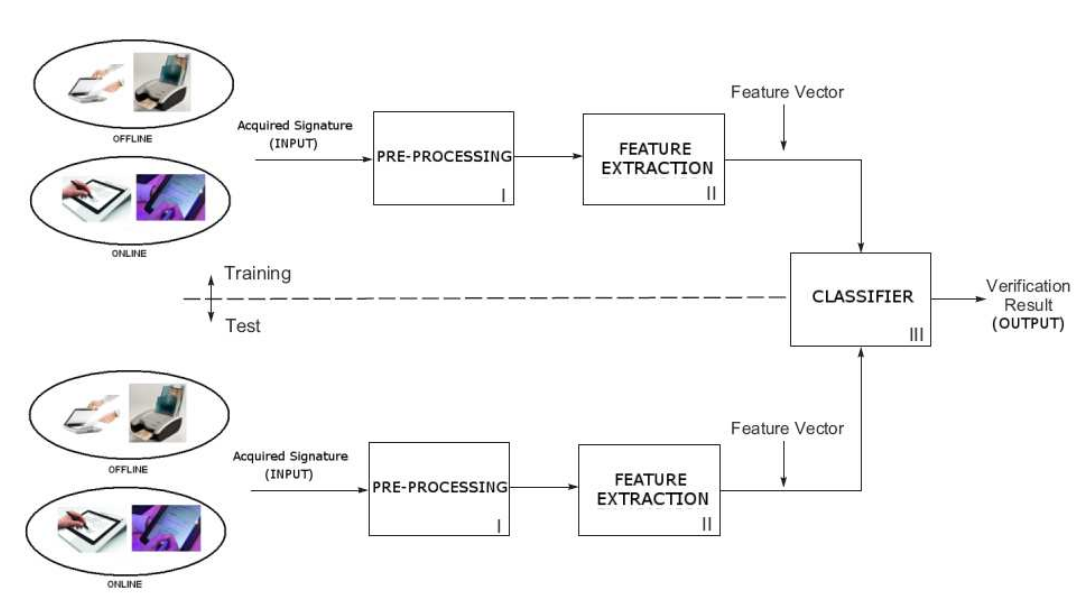
\includegraphics[width=0.65\textwidth]{imgs/vafm.png}
 \end{center}
\caption{Esquema de un sistema de VAFM. Fuente: \cite{tesis-parodi}.}
\label{fig:vafm}
\end{figure}

\begin{figure}[h!]
\begin{center}
 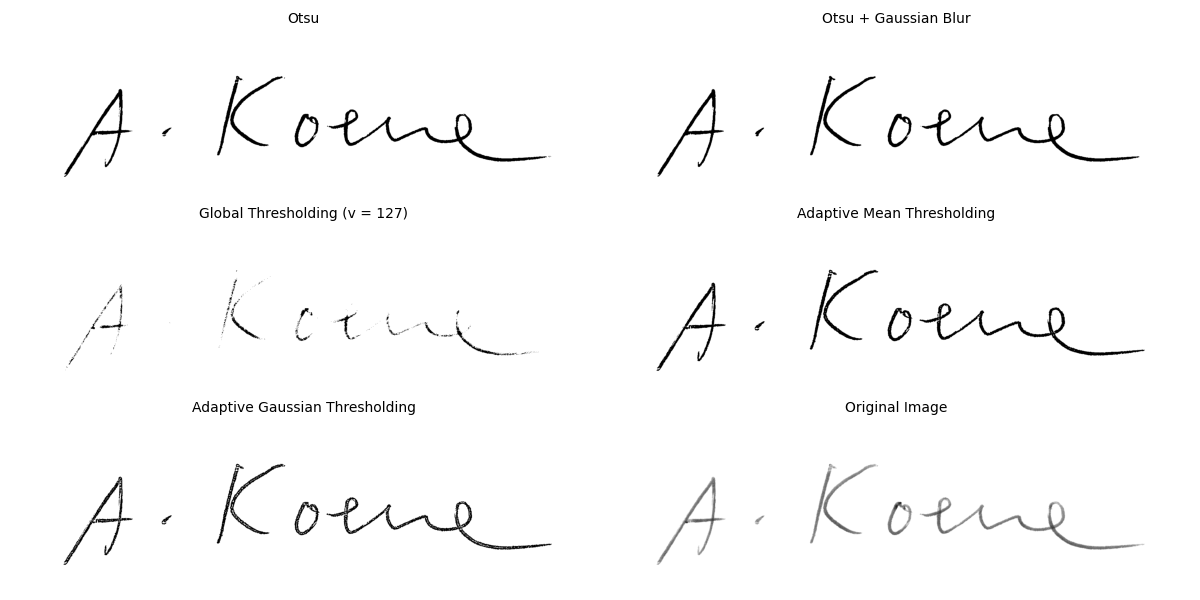
\includegraphics[width=0.9\textwidth]{imgs/image_binarization.png}
\end{center}
\caption{Distintas técnicas de preprocesamiento aplicadas a imágenes de firmas: binarización, filtros y normalización.}
\label{fig:preprocessing}
\end{figure}

Notar que se ha hecho hincapié en que este es el esquema \textit{clásico} de VAFM, entendiéndose por clásico como ``previo al Aprendizaje Profundo''. Como se explicó en la subsección \ref{subsection:representaciones}, el Aprendizaje Profundo revolucionó el paradigma del Aprendizaje Automatizado: ahora se suelen suministrar los datos crudos y es el algoritmo mismo quién aprende las características necesarias para el proceso de clasificación final.

La parte más crítica (con más impacto en los resultados) y que concentra la mayoría del conocimiento específico del dominio es la extracción de características. Es por ello que el trabajo de \cite{tesis-parodi} gira fundamentalmente en torno a esta fase.  En \cite{ip08} e \cite{ipp12} se propone gran variedad de características. La autora de \cite{tesis-parodi} ha propuesto contribuciones concernientes a la \textit{VAFM offline} en \cite{pg10a}, \cite{pg10b} y \cite{pgb11}.

\subsection{Extracción de características}

El objetivo de esta fase, que como se dijo suele ser la más importante, es encontrar una descripción adecuada de la firma.

Generalmente las características extraídas se basan en la geometría, tales como área, altura, ancho \cite{ayf90} \cite{spb94}, contorno \cite{np94}, orientación \cite{spb94}, dirección \cite{sd92}, \cite{dsg94} \cite{zna05}, la pendiente \cite{ayf90} y la curvatura \cite{jgc02} \cite{ksx04}. 

Las características descriptivas se suelen clasificar en \cite{tesis-parodi}:
\begin{itemize}
    \item \textbf{Globales:} consideran la firma como un todo. Son menos sensibles al ruido y a las variaciones de la firma \cite{hyw04}, lo cual lo hace una buen opción cuando se trabaja solamente con firmas auténticas \cite{tesis-parodi}.
    \item \textbf{Locales:} consideran partes especificas de la firma. Implica recurrir a técnicas de extracción más complejas \cite{mld11}, como por ejemplo utilizar grillas de segmentacion.
\end{itemize}

A partir de \cite{nr77} se han utilizado grillas para, a partir de ellas, extraer características locales, técnica también utilizada en \cite{sp86}, \cite{js01}, \cite{jybs00}, \cite{sjbs04}, \cite{jbs05}, \cite{ojfs05}, \cite{bzze13}.  

El trabajo de \cite{tesis-parodi} sigue esta línea proponiendo un método de grilla circular para la extracción de características locales. La idea de utilizar una grilla circular proviene de que resultan en menos sectores vacíos, además de poseer una estructura más apropiada en vistas de conseguir robustez respecto de la rotación de las firmas.

Las características propuestas en \cite{tesis-parodi} están basadas en los antecedentes de: \cite{jybs00} y \cite{js01} que utilizaron la densidad de píxeles (número de píxeles dentro de una celda), \cite{spb94} donde se calcula la distribución de píxles y \cite{jbs05} que propone utilizar el centro de gravedad (distancia del centro de gravedad en cada celda al centro de gravedad de toda la firma).

Escencialmente, \cite{tesis-parodi} ubica un esquema circular alrededor de la firma y la divide en $N$ sectores iguales, haciendo coincidir el centro de la grilla con el centro de masa de la firma (con esto se pretende la invariancia a la traslación). Luego extrae las siguientes características (ver figura \ref{fig:grillacircular}):\footnote{Notaremos $N$ el número de secciones circulares e $i$ a la $i$-ésima sección circular, con $i = 0, ..., N-1$. También referiremos con $R$ al radio de la grilla (distancia entre los dos puntos extremos).}

\begin{itemize}
    \item $x_{PD}$: Densidad de distribución de píxeles (en inglés, \textit{pixel density distributon})
    \begin{equation*}
    x_{PD_{i}} = \frac{\text{Número de píxeles negros de la sección }i}{\text{Número total de píxeles de la sección }i}
    \end{equation*}
    \item $x_{DGC}$: Distancia al centro de masa (en inglés, \textit{gravity center distance}).
    \begin{equation*}
    x_{DGC_{i}} = \frac{d_{GC_{i}}}{R}
    \end{equation*}
    Dividir por $R$ otorga cierta invarianza al escalado.
    \item $x_{AGC}$: Ángulo al centro de masa (en inglés, \textit{gravity center angle}).
    \begin{equation*}
        x_{AGC_{i}} = \frac{\alpha_{GC_{i}}}{\frac{2\pi}{N}}
    \end{equation*}
    Dividir por $\frac{2\pi}{N}$ no es estrictamente necesario, sino para lograr  escalar adecuadamente $\alpha_{GC}$ para diferentes $N$ (aunque nunca se trabajará con diferentes $N$ simultáneamente).
\end{itemize}

El vector característico es simplemente la concatenación de todas las características extraídas.

\begin{figure}[h!]
\begin{subfigure}{0.45\textwidth}
\begin{center}
 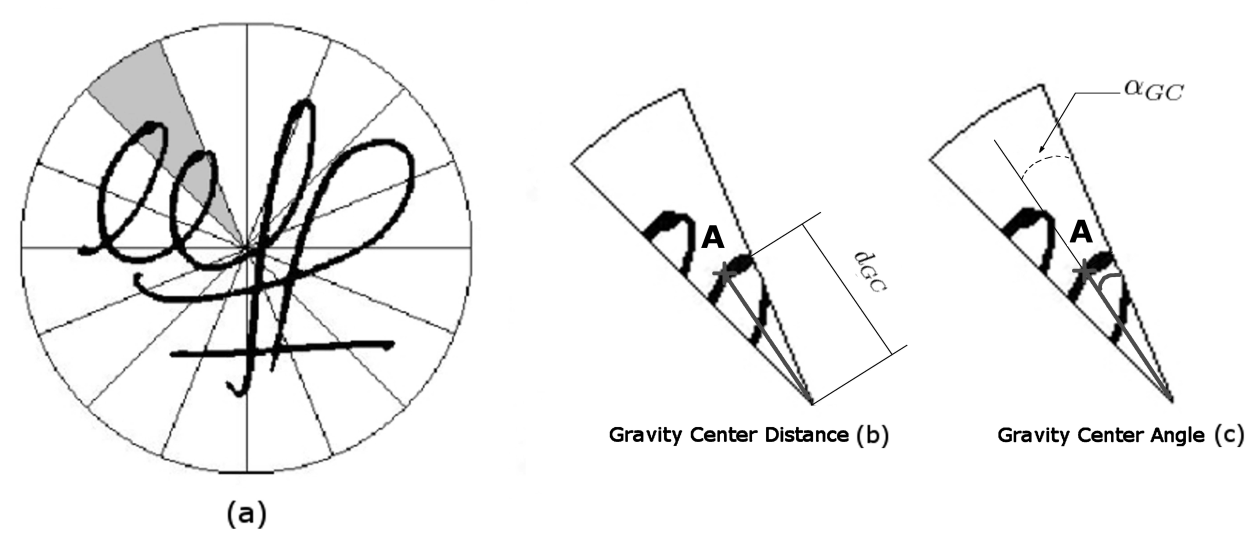
\includegraphics[width=0.85\textwidth]{imgs/grillacircular.png}
 \end{center}
\end{subfigure}
\caption{Esquema de grilla circular propuesto en  \cite{tesis-parodi}. (a) Se ha sombreado el sector analizado; (b) Distancia al centro de masa; (c) Ángulo del centro de masa. Fuente \cite{tesis-parodi}.}
\label{fig:grillacircular}
\end{figure}

\subsubsection{Invarianza rotacional mediante DFT}

Para lograr robustez frente a rotaciones, en \cite{tesis-parodi} se propone tomar los módulos de la Transformada Discreta de Fourier (DFT) de los vectores de características correspondientes a cada anillo de la grilla circular. Esta transformación produce características que son invariantes ante desplazamientos cíclicos de la secuencia original, lo cual equivale a rotaciones de la firma cuando el ángulo rotado es múltiplo de $\frac{2\pi}{N}$.

Sin embargo, cabe señalar una limitación de este enfoque: la invarianza obtenida es discreta, ya que solo se preserva ante rotaciones que correspondan exactamente al tamaño angular de una sección. Para valores pequeños de $N$ (es decir, pocas divisiones y por ende secciones angularmente grandes), las rotaciones típicas que pueden aparecer entre distintas instancias de una misma firma ---producto de variaciones en la inclinación al momento de firmar--- difícilmente coincidirán con múltiplos exactos del tamaño de sección. Esto sugiere que, en la práctica, el beneficio de esta técnica puede verse reducido cuando $N$ es pequeño.

Consideramos que el desarrollo de métodos que provean una invarianza rotacional más flexible podría resultar valioso, no solo para capturar la variabilidad intrapersonal en el ángulo de firmado, sino también porque habilitaría el uso de \textit{data augmentation} basada en rotaciones, permitiendo generar conjuntos de entrenamiento significativamente más grandes.

\subsection{Reutilizando las técnicas en nuestro problema}

\subsubsection{Entrenamiento de clasificadores y evaluación}

Recordar que en \cite{tesis-parodi} el problema a tratar consistía en verificar la identidad proclamada por el autor de cierta firma. Para ello, usa sobre dicha instancia un clasificador binario previamente entrenado para el autor que está siendo verificado, que determinará si la firma pertenece a la clase auténtica o falsa para dicha autoría. Cada clasificador (uno para cada autor) entrena la clase positiva utilizando firmas auténticas de dicho autor, y la clase negativa utilizando falsificaciones aleatorias (simuladas tomando firmas de otros autores). Esto último es muy importante debido a que, en un caso de uso real no se cuenta con falsificaciones al momento del entrenamiento. Se puede leer en detalle el protocolo de evaluación en la sección 3.5 de \cite{tesis-parodi}.

Como se dijo en la sección \ref{section:objectives}, nosotros queremos entrenar un clasificador para determinar si dos instancias de firmas son \textit{``la misma firma''} (fueron realizadas por el mismo autor). Notar que, potencialmente, los autores de las mencionadas firmas nunca han sido vistos con anterioridad por nuestro modelo. Es por ello que si bien reutilizaremos el proceso de extracción de catacterísticas con grilla circular de \cite{tesis-parodi}, no podemos entrenar un clasificador por autor.

Lo que haremos será entrenar un clasificador que reciba una combinación de las características de las imágenes de las dos firmas a analizar y determine si son o no la ``misma firma''. Para combinar los vectores característicos probaremos diferentes técnicas posibles tales como la diferencia vectorial o la concatenación de los vectores respectivos.  Nuestra metodología se explica con detalle en el capítulo siguiente, donde ahondaremos en el desarrollo de nuestros experimentos.

Nuestro problema es conceptualmente más complicado que el enfoque de \cite{tesis-parodi}, donde cada clasificador captura la varianza intrapersonal de un autor específico. La varianza intrapersonal puede diferir significativamente entre autores, por lo que construir un modelo que la capture en términos generales resulta mucho más difícil.

Más aún, la diferencia fundamental radica en que nuestra función de similaridad debe \textbf{extrapolar a autores no vistos durante el entrenamiento}. Mientras que en \textit{VAFM} se entrena un clasificador específico para cada autor (disponiendo de ejemplos de dicho autor), en nuestro caso el modelo debe aprender una noción de ``misma autoría'' lo suficientemente general como para aplicarse a firmas de personas que nunca formaron parte del conjunto de entrenamiento. Esta capacidad de generalización a nuevas identidades es lo que hace al problema intrínsecamente más difícil y lo emparenta con los problemas de \textit{One-Shot Learning} discutidos en la sección \ref{subsection:one-shot}.

\subsubsection{Métricas y convenciones}

Notar que tal como se ha explicado en la subsección \ref{subsubsection:metricasfirmas}, los conceptos $FAR$ y $FRR$ se encuentran invertidos en nuestro trabajo respecto a \cite{tesis-parodi}. Esto se debe a que nuestra clase positiva corresponde a cuando las firmas son \textit{no coincidentes} (al contrario de lo que ocurre con \cite{tesis-parodi}, donde la clase positiva concierne a que se verifica la identidad proclamada). Debemos tener en cuenta esto cuando analicemos lo resultados reportados en el mencionado trabajo para comprarlos con alguno de nuestros resultados.

Si nos fijamos en el resultado de $FAR$ de \cite{tesis-parodi}, es importante siempre considerar el respectivo a firmas ficticias, ya que como se explicó en \ref{subsection:categoria-firmas} en nuestro trabajo no utilizaremos falsificaciones simuladas.

Cabe aclarar, también, que se han utilizado conjunto de datos distintos (en el capítulo siguiente se ahondará sobre la elección y confección de los conjuntos de datos utilizados en nuestros experimentos). Y además, recalcar nuevamente que la metodología de evaluación y entrenamiento es diferente (evaluamos en firmas de autores no vistos en el entrenamiento), por lo cual el problema que nos proponemos resolver es conceptualmente mucho más difícil al de \textit{VAFM}.

\subsection{Resultados de \cite{tesis-parodi}}

Los resultados de \cite{tesis-parodi} correboran que la elección de grilla circular para el problema de \textit{VAFM} es ventajosa sobre la grilla rectangular. La grilla rectangular tiene buenos resultados de $FRR$ para número de subdivisiones grande ($N$ igual a 32, 64 o 128) pero peores resultados de $FAR$ sobre falsificaciones simples y entrenadas en dichos caso (es mejor par $N$ igual a 8). En cambio la grilla circular funciona bien en ambos casos para $N$ medianos ($N$ igual a 16), y luego empeora los resultados obtenidos al aumentar el número de subdivisiones. En \textit{tesis-parodi} se baraja la posibilidad de que esto se deba a que al aumentar las subdivisiones en la grilla circular el área de los sectores se reduce no uniformemente (al contrario de lo que sucede en la grilla rectangular). Como en nuestro trabajo no trabajaremos con falsificaciones simples (sólo con falsificaciones aleatorias como se dijo), consideraremos el grillado rectangular con $N$ grande ($N$ igual a 128), ya que en dicho casos muestra buenos resultados de $FAR$ en \cite{tesis-parodi}.

Finalmente los mejores resultados reportados en \cite{tesis-parodi} corresponden a las siguientes configuraciones:

\begin{table}[h!]
\begin{tabular}{l|c|c|l}
\cline{2-3}
\textbf{}                                              & \begin{tabular}[c]{@{}c@{}}Grilla circular\\ N=16, Kernal polinómico\end{tabular} & \begin{tabular}[c]{@{}c@{}}Grilla rectangular\\ N=128, Kernel RBF\end{tabular} &  \\ \cline{1-3}
\multicolumn{1}{|l|}{FRR}                              & 18.75 \%                                                                          & 27.875 \%                                                                      &  \\ \cline{1-3}
\multicolumn{1}{|l|}{FAR (firmas ficticias)}           & 0.0727 \%                                                                         & 0.0106 \%                                                                      &  \\ \cline{1-3}
\multicolumn{1}{|l|}{FAR (fals. simples y entrenadas)} & 2.125 \%                                                                          & 14.9167 \%                                                                     &  \\ \cline{1-3}
\end{tabular}
\end{table}

Nuestros objetivos, mencionados en \ref{subsubsection:costo-beneficio},



Notar que ninguno de los resultados exhibidos satisface (si bien está cerca) nuestra meta de lograr un \textit{recall} de al menos 0.8 y \textit{precision} de 0.95 mencionada en . De todos modo, cabe recordar las limitaciones expuestas en secciones anteriores sobre extrapolar los citados resultados a nuestro trabajo.

\subsubsection{Críticas metodológicas}

En los siguientes apartados expresamos algunas críticas al trabajo analizado. Entenderlas y analizarlas nos es útil para interpretar los resultados correctamente. Y también nos ha ayudado en el diseño correcto de nuestro protocolo de evaluación (capítulo siguiente).

\paragraph{Desbalance en el conjunto de datos de entrenamiento}\mbox{}\\

La clase verdadera de cada autor es entrenada con 14 firmas auténticas, mientras que la clase falsa es entrenada con firmas auténticas de otros autores.

El desbalance de clases es muy significativo y esto puede generar (depende de la configuración de entrenamiento de las SVM) un sesgo a favor de reducir el FAR sobre el FRR. Lamentablemente no tenemos acceso al código de los experimentos para constatar si se ha tomado alguna medida para mitigar el desbalance, como ponderar las clases a la hora de entrenar las SVM.

Este problem fue anoticiado por la autora en las conclusiones de la sección 3.9 \cite{tesis-parodi}.

\paragraph{Error metodológico en la evaluación de firmas ficticias}\mbox{}\\

El trabajo reporta resultados de $FAR$ para firmas ficticias. Para calcularlo utiliza firmas auténticas de los otros autores. Estas firmas provienen del conjunto de evaluación, o sea que no han sido utilizadas durante el entrenamiento.

Pese a que a primeras vistas puede parecer correcto tiene un sutil pero severo error: los autores de estas firmas sí han sido potencialmente usados para entrenar la clase falsa del clasificador que está siendo evaluado. Por lo qué el clasificador conoce firmas parecidas para la clase falsa. 

Naturalmente, esta correlación oculta podría no repetirse en un caso real. Ya que las falsificaciones simuladas no necesariamente se parecerán a ninguna de las firmas falsas que ha visto el clasificador durante el entrenamiento.

No podemos decir con certeza que no se hayan tomado recaudos frente a esta situación, como evaluar el $FAR$ de firmas ficticias para cada clasificador en autores que no se hayan utilizado para entrenar, porque no tenemos acceso al código de los experimentos. No obstante, como el protocolo de evaluación (sección 3.5 de \cite{tesis-parodi}) no hace salvedad alguna, pensamos que es probable que no se haya anoticiado de este error.

Es por este error que podemos sospechar que el $FAR$ de firmas ficticias es demasiado optimista.

\paragraph{Desbalance en el conjunto de datos de evaluación}\mbox{}\\

En la sección 3.5 de \cite{tesis-parodi} (\textit{``Protocolo de evaluación''}), se explica que para la fase de test se utilizan

\section{Conjuntos de datos}

\subsection{GPDS300}

Observaciones a su proceso de evaluación y conclusiones
En [TESIS-MARIANELA] se utilizó la base de datos GPDS300 Signature CORPUS [VFTA07]. Por regulaciones de la UE ya no se encuentra disponible para su uso. La base contaba con 160 escritore, 24 firmas auténticas y 30 falsificaciones por autor.


Fue el utilizado en \cite{tesis-parodi}. %Es presentado en \cite{vfta07}.

En [TESIS-MARIANELA] se utilizó la base de datos GPDS300 Signature CORPUS [VFTA07]. Por regulaciones de la UE ya no se encuentra disponible para su uso. En la página de GPDS (grupo de procesamiento de señales) existe actualmente un dataset sintético.
En la Conferencia Internacional sobre Análisis y Reconocimiento de Documentos (ICDAR por sus siglas en ingles) se han realizado competencias de vital importancia al área brindando a los investigadores la posibilidad de comparar el rendimiento de sus sistemas y proponer desafíos interesantes en sus datasets. 



La organización de estas competencias es de vital importancia para el área ya que
no sólo brinda a los investigadores la posibilidad de comparar el rendimiento de
sus sistemas, sino también de testear sus algoritmos con bases de datos estándar
y al alcance de toda la comunidad.
Además, las bases de datos presentadas en
el marco de las competencias suelen proponer desafíos interesantes. Por ejemplo,
para las competencias llevadas a cabo durante ICDAR 2009 y ICDAR 2011, se
construyó una base de datos conteniendo firmas de origen chino, mientras que
para la competencia llevada a cabo durante ICDAR 2013 se introdujo una base
de datos conteniendo firmas de origen japonés. Además de las competencias, en
los últimos años se organizaron distintos talleres y tutoriales en el marco de las
mencionadas conferencias. Estas reuniones periódicas permiten discutir los as-
pectos emergentes del área, brindándoles a los investigadores la oportunidad de
intercambiar ideas y discutir su trabajo actual en un contexto informal y disten-
didp.

Los primeros dos son de las competencias organizadas por ICDAR (International Conference on Document Analysis and Recognition).
La ventaja es que se consigue fácil tanto el dataset como el papper con los resultados. Ademas hay dando vueltas implementaciones (que no probé) de gente que se tiró a resolver esos dataset.
SigComp2011 tiene firmas occidentales (alemanas) y orientales (chinas) yo usaria solo las occidentales.
SigComp2009 tiene ~1800 firmas (entre autenticas y falsificaciones)
SigComp2011 tiene ~400 firmas occidentales (entre autenticas y falsificaciones).
Yo me tiraría a usar la 2009 porque tiene más. Aunque la otra es un poco más nueva.

La que usa Marianela en su tesis es GPDS960 pero no está disponible por una resolución de privacidad de la UE (ver la fuente). En internet tampoco la encontré (no busqué mucho tampoco).
La pagina sugiere usar las bases de datos sintéticas que listé abajo. A mí no me gustó el hecho de que sea sintética, aunque deben estar bien generadas, hay un paper y todo. Otro contra es que hay que llenar un formulario y mandarlo, no es tan simple como poner descargar. Lo bueno de esa opción es que son muchísimas como 4000.
Tampoco pude encontrar gratis el papper de este último dataset "Off-line handwritten SignatureGPDS-960 Corpus." F. Vargas, M.A. Ferrer, C.M. Travieso, and J.B. Alonso.


Los conjuntos de datos utilizados Sigcomp 2009 \cite{sigcomp2009} y Sigcomp 2011 \cite{sigcomp2009}, provienen de las competencias llevadas a cabo durante las ediciones 2009 y 2011 respectivamente de la International Conference on
Document Analysis and Recognition (ICDAR).

Las competencias presentan base de datos interesantes y permiten a los investigadores del área la posibilidad de comparar su rendimiento de manera estándar \cite{tesis-parodi}.



\section{Problemas de similitud}

\subsection{Problemas clásicos similares: \textit{Face Recognition} y \textit{Face Verification}}

Los rostros, al igual que las firmas, son una característica biométrica que puede ser utilizada para la autenticación. No es de sorprender, entonces, que los mismos problemas que atañen a firmas tengan su paralelismo con el procesamiento de imágenes de rostros. En ambos casos resulta fundamental extraer características discriminativas que permitan clasificar o comparar instancias provenientes de distintas personas.

El problema de \textbf{\textit{Face Verification}} consiste en verificar si un cierto rostro pertenece a una determinada persona (de la cual se conocen rostros). La entrada es una imagen del rostro junto con la identidad declarada, y la salida del modelo es un booleano indicando si la imagen corresponde efectivamente a dicha persona:

\begin{equation*}
    Face \ Verification \ System (face\_image, \ person\_id ) : Bool
\end{equation*}

En contraste, en el problema de \textit{\textbf{Face Recognition}} sólo se posee una imagen y se debe detectar si el rostro corresponde a alguna persona de una base de datos de rostros conocidos. Es decir, la entrada es únicamente la imagen del rostro y la salida es la identidad correspondiente (o ``no reconocido'' si no coincide con ninguno de la base de datos):

\begin{equation*}
    Face \ Recognition \ System (face\_image) :  Person \ ID \cup \{ Not\ Recognized \}
\end{equation*}

Notar que si bien el problema de \textit{Face Recognition} parece más difícil que el de \textit{Face Verification}, una solución a este último con suficiente precisión, se puede trasladar al segundo iterando para identidad posible de la base de datos.

\subsection{\textit{One-Shot Learning}} \label{subsection:one-shot}

La mayor dificultad de ambos problemas es que generalmente consisten en problemas de \textbf{\textit{One-Shot learning}} (o \textit{Few-Shot learning}):
\begin{itemize}
    \item El conjunto de entrenamiento cuenta con un (o unos pocos) ejemplos para cada categoría (persona o identidad en el caso de rostros).
    \item Existen a su vez muchas etiquetas (muchas personas distintas). Y además pueden agregarse nuevas e idealmente no queremos re-entrenar todo el modelo cada vez que esto ocurra.
\end{itemize}
De estas restricciones se desprende que no será útil atacar el problema utilizando un clasificador donde haya una clase por identidad, ya que al poseer pocos ejemplos de cada clase, el entrenamiento lograría una muy pobre precisión. Además, este enfoque obligaría a re-entrenar el modelo cada vez que se quiera agregar una nueva persona. \\
En vez de esto, una solución posible es aprender una función de similaridad $d$:
\begin{equation*}
    d(img_1, img_2) = \text{grado de diferencia entre ambas personas}
\end{equation*}
Luego, podemos resolver \textit{Face Verification} comparando la salida de $d$ respecto de un umbral $\tau$: 

\begin{equation*}
    d(img_1, img_2) \left\{ \begin{array}{lcc}
             \leq \tau &   si  & id(img_1) = id(img_2) \\
             \\ > \tau &   si  & id(img_1) \neq id(img_2) 
             \end{array}
   \right.
\end{equation*}

De este modo resolvemos un problema ``más fácil'' que el de reconocer la identidad de cada sujeto (el modelo tiene disponible en su valuación la imágen contra la cuál está comparando). 

Además, con este enfoque de aprender una función de similaridad de rostros $d$ generalizable a identidades no vistas sobre el entrenamiento, no necesitaremos re-entrenar el modelo de agregarse nuevas personas a la base de datos.

\subsection{\textit{Redes Siamesas}}

La arquitectura que se emplea para esta clase de problemas es conocida como \textbf{\textit{Redes Siamesas}} \cite{siamess-lecun}. Consiste en utilizar una red convolucional clásica (una sucesión de convoluciones y capas de \textit{pooling}) y valerse de las activaciones de entrada de la última capa (la predicción) como vector de características (también llamado \textbf{\textit{embedding}} o \textbf{\textit{encoding}} de la imagen). Para finalmente calcular la similitud como la distancia entre ambos \textit{embeddings}. Ver figura \ref{img:siamess}. En la figura \ref{fig:signatures_paired} se muestra un ejemplo de cómo se estructura un dataset pareado para entrenar estas redes.

\begin{figure}[h]
\centering
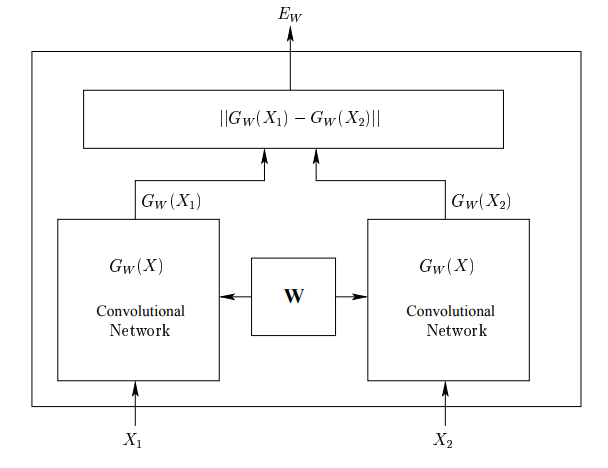
\includegraphics[width=0.7\textwidth]{imgs/siamess.png}
\caption{Arquitectura general de una \textit{Red Siamesa}. Fuente: \cite{siamess-lecun}}
\label{img:siamess}
\end{figure}

\begin{figure}[h]
\centering
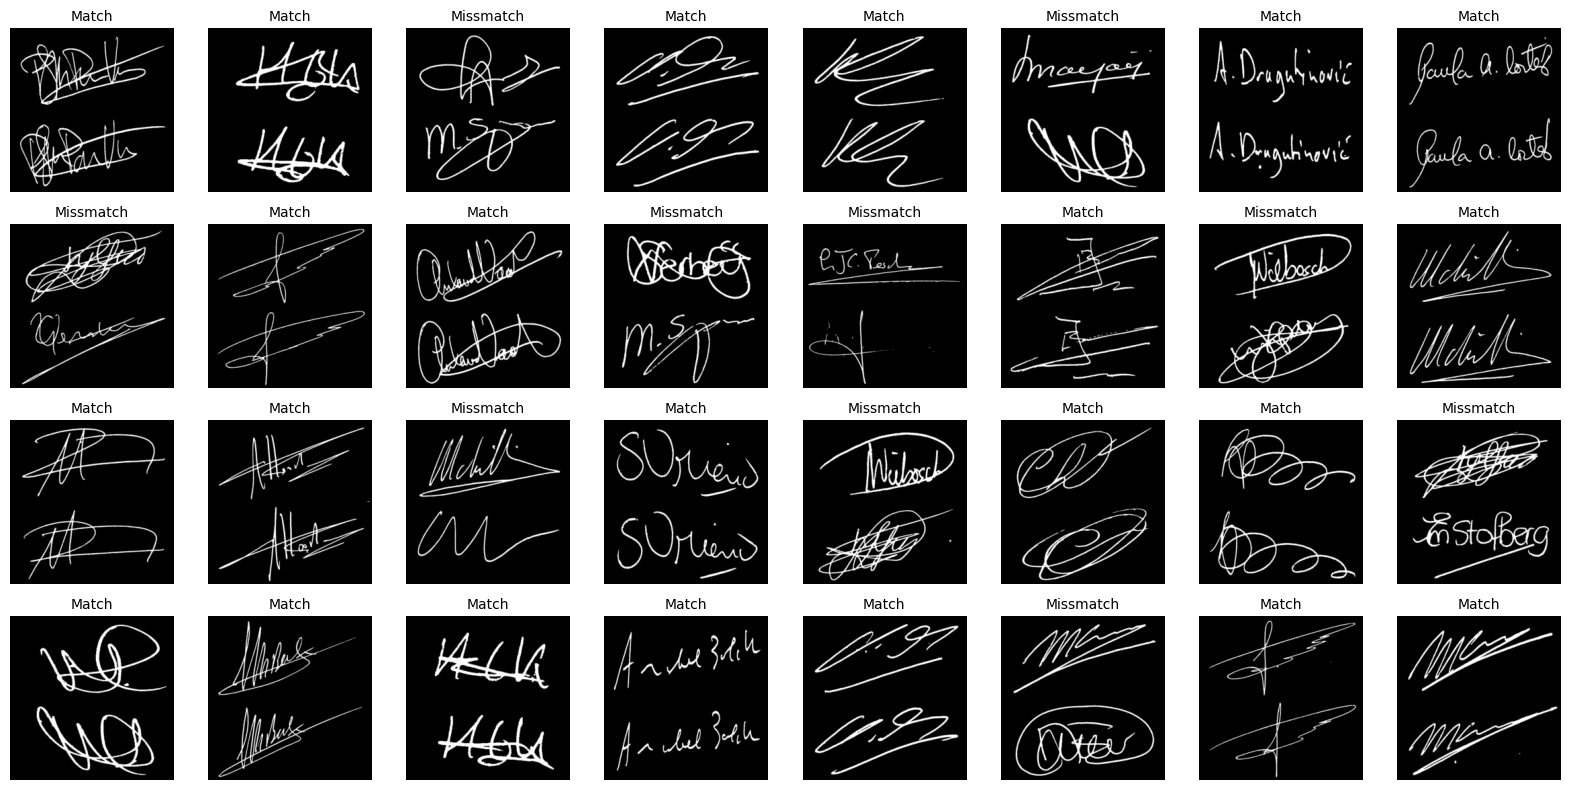
\includegraphics[width=0.9\textwidth]{imgs/signatures_paired.png}
\caption{Ejemplo de un dataset pareado de firmas: cada instancia consiste en un par de firmas junto con un veredicto indicando si corresponden o no al mismo autor.}
\label{fig:signatures_paired}
\end{figure}

Notar que en el cálculo de los \textit{embeddings} de ambas imágenes se utilizan los mismos pesos (notado como $W$ en la figura \ref{img:siamess}). Esta técnica dónde los mismos parámetros se reutilizan, en dos o más cómputos diferentes, en cada evaluación del modelo, se suele denominar \textit{Tied Weights} en la jerga del \textit{aprendizaje profundo}.


En línea con la figura \ref{img:siamess}, notaremos con $G_W$ la función definida al aplicar nuestro modelo (también llamado \textit{encoder}). Siendo  entonces $G_W(img)$ el \textit{encoding} o \textit{embedding} de la imagen $img$ utilizada.

Para comparar los \textit{embeddings} pueden utilizarse diferentes funciones distancia (la distancia coseno, la euclídea y $\mathcal{X}^2$ están entre las más escogidas). 

El entrenamiento debiera optimizar el \textit{encoder} $G_W$, hallando valores de $W$ óptimos, para extraer características útiles a la hora de comparar dos imágenes (rostros en el caso del problema de \textit{Face Verification}). Notar que este es un claro ejemplo de lo discutido en \ref{subsection:representaciones} donde se utiliza redes neuronales para aprender las características útiles a extraer, en vez de codificarlas a mano (las cuáles probablemente son dependiente del dominio de las imágenes a comparar).
Más formalmente, el entrenamiento deberá aprender parámetros del \textit{encoder} tal que:
\begin{equation*}
    ||~G_W(img_1) - G_W(img_2)~||_2 < \tau \Longleftrightarrow{} \text{id}(img_1) = \text{id}(img_2) 
\end{equation*}

Notar la importancia para el desarrollo del \textit{Aprendizaje Profundo} de la funcionalidad de diferenciación automática (también llamada \textbf{\textit{Autograd}}) de los \textit{frameworks} como \textit{Pytorch} o \textit{TensorFlow}: cuestiones como \textit{Tied Weights} en la formulación del costo hacen que las expresiones de los gradientes sean complicadas de tener que calculárselas manualmente. Afortunadamente, las librerías encapsulan dicho problema y los mismos son computados automáticamente. Lo que da pie a que se experimente con formulaciones más complejas y da lugar a entrenamientos más sofisticados.

\subsection{}

Resta definir la función de costo

\subsection{\textit{Image Similarity}}

\subsection{\textit{Omniglot Dataset}}
